% Options for packages loaded elsewhere
\PassOptionsToPackage{unicode}{hyperref}
\PassOptionsToPackage{hyphens}{url}
%
\documentclass[
]{article}
\usepackage{lmodern}
\usepackage{amssymb,amsmath}
\usepackage{ifxetex,ifluatex}
\ifnum 0\ifxetex 1\fi\ifluatex 1\fi=0 % if pdftex
  \usepackage[T1]{fontenc}
  \usepackage[utf8]{inputenc}
  \usepackage{textcomp} % provide euro and other symbols
\else % if luatex or xetex
  \usepackage{unicode-math}
  \defaultfontfeatures{Scale=MatchLowercase}
  \defaultfontfeatures[\rmfamily]{Ligatures=TeX,Scale=1}
\fi
% Use upquote if available, for straight quotes in verbatim environments
\IfFileExists{upquote.sty}{\usepackage{upquote}}{}
\IfFileExists{microtype.sty}{% use microtype if available
  \usepackage[]{microtype}
  \UseMicrotypeSet[protrusion]{basicmath} % disable protrusion for tt fonts
}{}
\makeatletter
\@ifundefined{KOMAClassName}{% if non-KOMA class
  \IfFileExists{parskip.sty}{%
    \usepackage{parskip}
  }{% else
    \setlength{\parindent}{0pt}
    \setlength{\parskip}{6pt plus 2pt minus 1pt}}
}{% if KOMA class
  \KOMAoptions{parskip=half}}
\makeatother
\usepackage{xcolor}
\IfFileExists{xurl.sty}{\usepackage{xurl}}{} % add URL line breaks if available
\IfFileExists{bookmark.sty}{\usepackage{bookmark}}{\usepackage{hyperref}}
\hypersetup{
  pdftitle={batMods},
  pdfauthor={AM},
  hidelinks,
  pdfcreator={LaTeX via pandoc}}
\urlstyle{same} % disable monospaced font for URLs
\usepackage[margin=1in]{geometry}
\usepackage{graphicx}
\makeatletter
\def\maxwidth{\ifdim\Gin@nat@width>\linewidth\linewidth\else\Gin@nat@width\fi}
\def\maxheight{\ifdim\Gin@nat@height>\textheight\textheight\else\Gin@nat@height\fi}
\makeatother
% Scale images if necessary, so that they will not overflow the page
% margins by default, and it is still possible to overwrite the defaults
% using explicit options in \includegraphics[width, height, ...]{}
\setkeys{Gin}{width=\maxwidth,height=\maxheight,keepaspectratio}
% Set default figure placement to htbp
\makeatletter
\def\fps@figure{htbp}
\makeatother
\setlength{\emergencystretch}{3em} % prevent overfull lines
\providecommand{\tightlist}{%
  \setlength{\itemsep}{0pt}\setlength{\parskip}{0pt}}
\setcounter{secnumdepth}{-\maxdimen} % remove section numbering
\usepackage{booktabs}
\usepackage{longtable}
\usepackage{array}
\usepackage{multirow}
\usepackage{wrapfig}
\usepackage{float}
\usepackage{colortbl}
\usepackage{pdflscape}
\usepackage{tabu}
\usepackage{threeparttable}
\usepackage{threeparttablex}
\usepackage[normalem]{ulem}
\usepackage{makecell}
\usepackage{xcolor}
\newlength{\cslhangindent}
\setlength{\cslhangindent}{1.5em}
\newenvironment{cslreferences}%
  {\setlength{\parindent}{0pt}%
  \everypar{\setlength{\hangindent}{\cslhangindent}}\ignorespaces}%
  {\par}

\title{batMods}
\author{AM}
\date{28 June, 2020}

\begin{document}
\maketitle

This is an overview of an R package I am currently developing as part of
a research paper looking into virus dynamics in bat populations of
Australia.

The link to the github repo is:
\url{https://github.com/aaronm70/batMods}, which contains all code and
associated data.

\hypertarget{overview}{%
\section{Overview}\label{overview}}

batMods fits a number of discrete time stochastic models of varying
structures with and without seasonal forces, to observed bat virus data
(currently from boonah australia (Field et al. 2015)), using particle
MCMC based methods. The goal is to identify which dynamical model best
represents the observed viral samples from wild populations and gain
further insight into between-host viral dynamics in bats. Model
comparison is conducted using an approximate leave one out cross
validation algorithm, incorporating Pareto smoothed importance sampling
(Vehtari et al. 2019). This algorithm uses pointwise likelihood values
to compute the log pointwise predictive density and its Monte Carlo
standard error, the effective number of parameters, Pareto k diagnostic
values (which can help assess if a model is well specified) and an
information criterion ``looic'' (lower values suggest a better model
fit). (Vehtari, Gelman, and Gabry 2017a, 2017b; Vehtari et al. 2015).

\begin{figure}
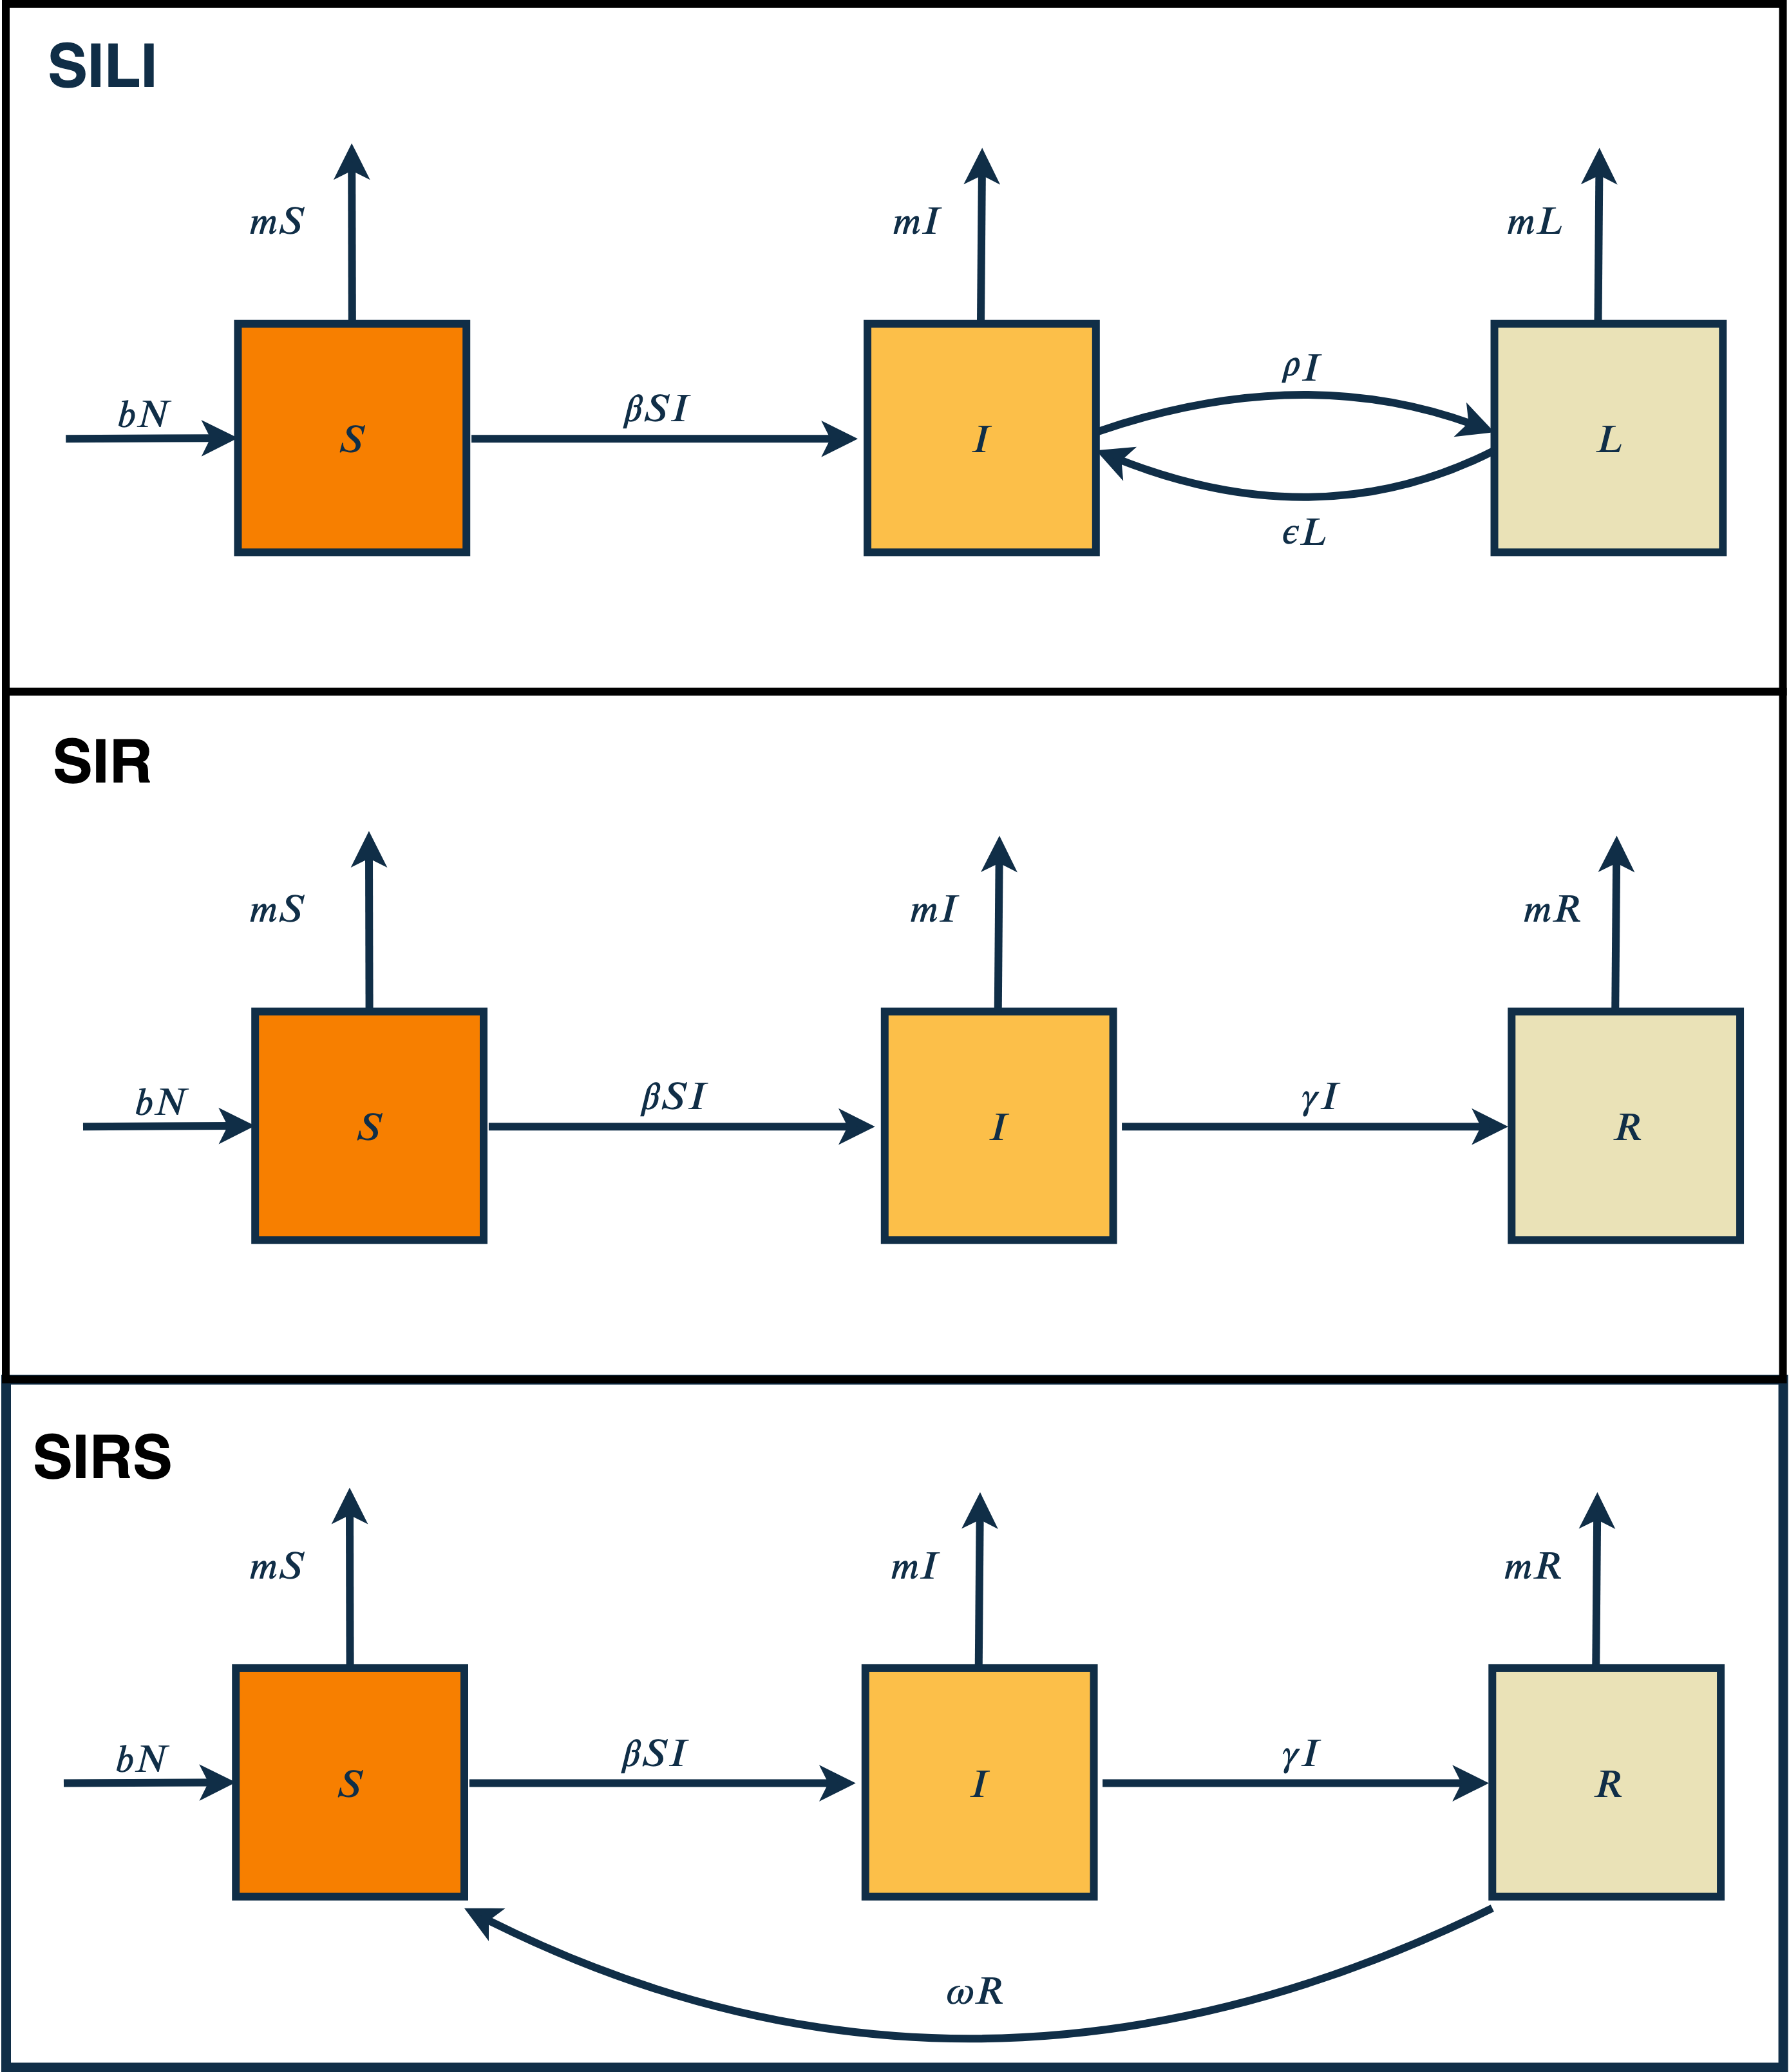
\includegraphics[width=1\linewidth,height=0.75\textheight]{https://github.com/aaronm70/batMods/blob/master/figures/adultMod-Paper} \caption{Figure 1: Model structures for SILI, SIR and SIRS type models, each model is built on top of an age structured bat population model and transitions occur between variable states as probablistic draws from binoial distributions, see suppplementary materials for full details}\label{fig:unnamed-chunk-1}
\end{figure}

\begin{itemize}
\item
  Currently batMods fits three primary models structures with and
  without maternal immmunity and seasonal forces (figure 1) to multiple
  data-types, including serology and PCR data.
\item
  The analysis can be run from the runscript.R file.
\item
  The metropilis hastings and particle filter algorithms run in R,
  whilst the model itself runs in C code, which is implemented via the
  Odin package.
\item
  The model and fitting methods are described in modelMethods.pdf
  \url{https://github.com/aaronm70/batMods/blob/master/modelMethods.pdf}
\item
  This is a work in progress as part of a paper on bat virus dynamics,
  as such should not be seen as a final analysis
\end{itemize}

\hypertarget{references}{%
\section*{References}\label{references}}
\addcontentsline{toc}{section}{References}

\hypertarget{refs}{}
\begin{cslreferences}
\leavevmode\hypertarget{ref-field2015spatiotemporal}{}%
Field, Hume, David Jordan, Daniel Edson, Stephen Morris, Debra Melville,
Kerryn Parry-Jones, Alice Broos, et al. 2015. ``Spatiotemporal Aspects
of Hendra Virus Infection in Pteropid Bats (Flying-Foxes) in Eastern
Australia.'' \emph{PloS One} 10 (12): e0144055.

\leavevmode\hypertarget{ref-VehtariLooPackage}{}%
Vehtari, Aki, Jonah Gabry, Mans Magnusson, Yuling Yao, and Andrew
Gelman. 2019. ``Loo: Efficient Leave-One-Out Cross-Validation and Waic
for Bayesian Models.'' \url{https://mc-stan.org/loo}.

\leavevmode\hypertarget{ref-vehtari2017practical}{}%
Vehtari, Aki, Andrew Gelman, and Jonah Gabry. 2017a. ``Practical
Bayesian Model Evaluation Using Leave-One-Out Cross-Validation and
Waic.'' \emph{Statistics and Computing} 27 (5): 1413--32.

\leavevmode\hypertarget{ref-AkiLoo}{}%
---------. 2017b. ``Practical Bayesian Model Evaluation Using
Leave-One-Out Cross-Validation and Waic.'' \emph{Statistics and
Computing} 27 (5): 1413--32.
\url{https://doi.org/10.1007/s11222-016-9696-4}.

\leavevmode\hypertarget{ref-vehtari2015pareto}{}%
Vehtari, Aki, Daniel Simpson, Andrew Gelman, Yuling Yao, and Jonah
Gabry. 2015. ``Pareto Smoothed Importance Sampling.'' \emph{arXiv
Preprint arXiv:1507.02646}.
\end{cslreferences}

\end{document}
